% ====================== main.tex ======================
\documentclass[man,12pt,letterpaper,donotrepeattitle,floatsintext]{apa7}

\usepackage[american]{babel}
\usepackage[utf8]{inputenc}
\usepackage[T1]{fontenc}

% Times-like font (APA 7 compliant)
\usepackage{newtxtext,newtxmath}

% Double spacing
\usepackage{setspace}
\doublespacing

% Nice URLs and clickable links (without colored boxes)
\usepackage{url}

% APA citations - natbib mode for \citep command
\usepackage[natbibapa]{apacite}

% Configure hyperref (already loaded by apa7/apacite)
\hypersetup{hidelinks}

% Python syntax highlighting for code listings
\usepackage{pdfpages}
\usepackage{listings}
\usepackage{xcolor}

% Define Python style for listings
\lstdefinestyle{pythonstyle}{
    language=Python,
    basicstyle=\ttfamily\footnotesize\linespread{1}\selectfont,
    keywordstyle=\color{blue}\bfseries,
    stringstyle=\color{red},
    commentstyle=\color{green!60!black}\itshape,
    numberstyle=\tiny\color{gray},
    numbers=left,
    numbersep=8pt,
    stepnumber=1,
    showstringspaces=false,
    breaklines=true,
    frame=single,
    rulecolor=\color{black!30},
    backgroundcolor=\color{gray!5},
    tabsize=4,
    captionpos=b,
    xleftmargin=2em,
    framexleftmargin=1.5em,
    morekeywords={self,True,False,None},
    aboveskip=1em,
    belowskip=1em,
}

% =============================================
% Title-page information – NEW apa7 syntax (2022+)
% =============================================
\title{AI-Generated Image Detection: A Comparative Study of CNN Architectures}
\shorttitle{AI-Generated Image Detection}

\authorsnames{Marston Ward, Victor Salcedo, Jasper Dolar}
\authorsaffiliations{{University of San Diego}}

\course{Applied Artificial Intelligence: Computer Vision}
\professor{Professor Roozbeh Sadeghian}
\duedate{December 8, 2025}

% Optional
\abstract{%
  This study evaluates three deep learning architectures for detecting AI-generated images: 
  a custom convolutional neural network (CNN), ResNet50, and EfficientNet-B2. Using a 
  dataset of 152,710 images from Hugging Face, we trained and compared these models to 
  identify synthetic visual content. The custom CNN served as a baseline, while ResNet50 
  and EfficientNet-B2 employed transfer learning with frozen pretrained backbones. Results 
  demonstrate that transfer learning architectures significantly outperform the baseline 
  CNN, with EfficientNet-B2 achieving the highest test accuracy. This work provides practical 
  insights into model selection for deepfake detection applications, balancing accuracy, 
  computational efficiency, and deployment considerations.
}

\keywords{deepfake detection, AI-generated images, convolutional neural networks, transfer learning, ResNet50, EfficientNet}

% =============================================
\begin{document}

% Override APA7 caption formatting for centered captions
\captionsetup[table]{
  format=plain,
  labelsep=period,
  justification=centering,
  singlelinecheck=false,
  font={normalsize,bf}
}

% Custom Title Page
\begin{titlepage}
    \centering
    {\LARGE\bfseries AI-Generated Image Detection: A Comparative Study of CNN Architectures\par}
    \vspace{1.5cm}
    {\large Marston Ward, Victor Salcedo, Jasper Dolar\par}
    \vspace{0.5cm}
    {\large University of San Diego\par}
    \vspace{0.5cm}
    {\large Applied Artificial Intelligence: Computer Vision\par}
    \vspace{0.5cm}
    {\large Professor Roozbeh Sadeghian\par}
    \vspace{0.5cm}
    {\large December 8, 2025\par}
    \vfill
\end{titlepage}


% Abstract goes on its own page in manuscript format
\thispagestyle{empty}
\newpage

% ================== Main content ==================
\section{Introduction}
The rapid proliferation of artificially generated images and videos, 
collectively known as deepfakes, presents a critical challenge to digital integrity, 
as this fabricated content is increasingly misrepresented as authentic 
\citep{Kingsley2024, Maharjan2023}. This surge in fraud and deception directly
necessitates the development of highly reliable deepfake detection methods capable 
of accurately distinguishing genuine visual media from sophisticated manipulation 
\citep{ST2022}. Deepfake technology leverages advanced machine learning techniques, 
predominantly Generative Adversarial Networks (GANs), to create synthetic media 
that convincingly mimics real-world auditory and visual content 
\citep{Kingsley2024, Maharjan2023}. The relative ease of generating such convincing 
deepfakes underscores the urgency of establishing robust, responsive detection systems.

Recent progress in deep learning, particularly utilizing Convolutional Neural Networks 
(CNNs), has proven effective in tackling the complexity of deepfake content. 
Research has demonstrated the efficacy of combining CNNs with Long Short-Term Memory 
(LSTM) networks for detecting deepfake videos, highlighting the crucial role of these 
integrated systems in combating digital misinformation \citep{Abidin2022, Gawali2024}. 
Similarly, the application of high-performance models, like the EfficientNet architecture, 
has led to significant improvements in detection accuracy \citep{Sowmya2024}. 
Furthermore, advanced approaches that integrate CNNs with specialized texture variation 
networks have been shown to effectively analyze inherent texture features to distinguish 
between real and manipulated images (Haseena et al., 2023).

This study aims to explore the foundational principles of deepfake detection by 
focusing on AI-generated images using a CNN model. Specifically, this work introduces 
the methodology of fine-tuning the established ResNet50 architecture \citep{He2016} to 
illustrate core concepts in deepfake identification. A critical element for the successful 
training of any deepfake detection model is access to extensive, high-quality datasets, 
many of which are now openly available on platforms such as Hugging Face \citep{HuggingFace}. 
As \cite{Berrahal2023} emphasizes, a detailed understanding of dataset characteristics, 
including its composition and the technology used to generate the synthetic images, 
is fundamental for developing effective detection methodologies. Utilizing larger and 
more diverse training datasets is known to significantly enhance model performance, 
which is particularly vital for real-world applications where the variance of 
deepfakes is high \citep{Frid-Adar2018, Golilarz2024}.

In summary, the detection of deepfake images presents an ongoing and complex 
challenge, driven by the continuous and rapid advancement of synthetic media 
generation technology. The strategic integration of state-of-the-art deep learning 
methods, particularly robust CNN architectures and GANs, combined with comprehensive, 
large-scale training datasets, represents the most strategic path toward developing 
effective detection systems. As this technological arms race progresses, continuous 
refinement of both research and methodology remains pivotal in mitigating the severe 
detrimental impacts of deepfake technology \citep{Berrahal2023, Haseena2023}.


\section{Exploratory Data Analysis (EDA)}
\label{eda}
This project uses a large-scale image dataset from Hugging Face containing 152,710 
images labeled as real or AI-generated. A quick inspection confirmed that each entry 
includes an image and a binary label, with 0 for real and 1 for AI-generated. Initial 
visualization of random samples showed that the dataset loaded correctly and contained 
a wide range of subjects, resolutions, and styles, which is appropriate for a general 
image classification task.

A histogram of label frequencies showed an even distribution between the two classes. 
This balance reduces the risk of biased decision boundaries and allows the model to 
learn useful visual patterns rather than defaulting to a majority class. Visual 
exploration also revealed high diversity across both categories, including animals, 
portraits, objects, and scenes, suggesting that the model would need to rely on structural
and textural cues associated with generated images rather than on semantic content.

The raw images varied in size, aspect ratio, and color format, so all samples were 
standardized to 224 by 224 pixels and converted to a three-channel RGB. This ensured 
consistent input dimensions for both the CNN and the pre-trained ResNet model and 
aligned with ImageNet-based normalization. Visual checks after transformation 
confirmed that important features were preserved while enforcing a uniform $224 \times 224 \times 3$ 
shape for stable training.

After pre-processing, the dataset was shuffled and split into training, validation, 
and test sets at an 80, 10, and 10\% ratio, producing 122,168 training images 
and 15,271 images each for validation and testing. These volumes are large enough 
to support deep learning and improve generalization across unseen AI-generation styles. 
DataLoader verification confirmed that batches were formed correctly, labels matched 
the right images, and normalization could be reversed for visualization, 
indicating that the pipeline was functioning as intended.

Overall, the EDA demonstrated that the dataset is balanced, diverse, and well-suited 
for convolutional modeling. The image inspections showed clear visual differences 
between real and generated content, and the preprocessing steps produced a stable, 
consistent input format. These findings confirmed that the data was ready for model 
development and that the classification task was appropriate for deep learning methods.

\section{Methodology}
\label{methodology}

We implemented and compared three distinct architectures to evaluate their effectiveness 
in detecting AI-generated images: a custom CNN built from scratch, ResNet50 with transfer 
learning, and EfficientNet-B2 with transfer learning.

\subsection{Custom CNN Architecture}
The baseline model consisted of three convolutional blocks, each containing a convolutional 
layer, batch normalization, ReLU activation, and max pooling. The architecture progressively 
increased feature maps from 32 to 128 channels while reducing spatial dimensions through 
pooling. A fully connected classifier with dropout (0.5) was used for regularization. 
This model output a single logit for binary classification using BCEWithLogitsLoss, 
totaling approximately 2.1 million trainable parameters. The custom CNN was trained 
for 10 epochs with an Adam optimizer (learning rate 0.001).

\subsection{ResNet50 Transfer Learning}
The ResNet50 model employed a pretrained backbone from ImageNet with all convolutional 
layers frozen to preserve learned features. Only the final fully connected layer was 
replaced with a 2-class classifier and trained using CrossEntropyLoss. This approach 
dramatically reduced trainable parameters to approximately 2,000 while leveraging the 
deep residual architecture's 25.6 million pretrained weights. Training used an Adam 
optimizer with learning rate $1 \times 10^{-4}$ and weight decay $1 \times 10^{-4}$ 
for 5 epochs.

\subsection{EfficientNet-B2 Transfer Learning}
EfficientNet-B2 utilized compound scaling to balance network depth, width, and resolution 
efficiently. Similar to ResNet50, the pretrained backbone was frozen while the classifier 
head was retrained for binary classification. This model contained approximately 9.1 million 
total parameters with only the final classifier layers being trainable. Training configuration 
matched ResNet50 with 5 epochs and identical optimization parameters.

\subsection{Training Configuration}
All models were trained on an A100 GPU using automatic mixed precision (AMP) for computational 
efficiency. Data augmentation during training included random horizontal flips, random rotation 
($\pm$10$^\circ$), and color jittering (brightness, contrast, saturation, hue). Images were resized to 
224 $\times$ 224 pixels and normalized using ImageNet statistics. The dataset was split 80/10/10 for 
training, validation, and testing, with batch size 32 and 2 workers for data loading. 
Models were evaluated on a held-out test set of 15,271 images.

\section{Results}
\label{results}

Table~\ref{tab:results} summarizes the test accuracy for all three architectures. 
EfficientNet-B2 achieved the highest performance, followed closely by ResNet50, while 
the custom CNN provided competitive baseline results despite its simpler architecture.

\processdelayedfloats
\begin{table}[!htbp]
\centering
\captionsetup{justification=centering}
\begin{threeparttable}
\caption{Model Performance Comparison}
\label{tab:results}
\begin{tabular}{lcc}
\hline
\textbf{Model} & \textbf{Test Accuracy} & \textbf{Trainable Parameters} \\
\hline
Custom CNN & 85.2\% & 2.1M \\
ResNet50 & 92.7\% & 2K \\
EfficientNet-B2 & 94.1\% & 7.8M \\
\hline
\end{tabular}
\end{threeparttable}
\end{table}

The transfer learning approaches demonstrated superior performance with significantly 
fewer trainable parameters compared to the custom CNN. ResNet50's frozen backbone strategy 
proved highly effective, achieving competitive accuracy while training only the final 
classification layer. EfficientNet-B2's compound scaling and efficient architecture 
design yielded the best overall results, validating its effectiveness for high-resolution 
image classification tasks.

Training efficiency varied considerably across models. The custom CNN required 10 epochs 
and approximately 2-3 minutes per epoch. Transfer learning models converged faster with 
only 5 epochs needed, though ResNet50 took 3-5 minutes per epoch and EfficientNet-B2 
required 4-6 minutes per epoch due to their deeper architectures.

\section{Discussion and Conclusion}
\label{conclusion}

This study demonstrated that transfer learning architectures significantly outperform 
baseline CNNs for AI-generated image detection. The pretrained features from ImageNet 
proved highly transferable to synthetic image detection, enabling effective classification 
with minimal fine-tuning. EfficientNet-B2's superior performance (94.1\% test accuracy) validates compound 
scaling as an effective approach for balancing model capacity and computational efficiency. ResNet50 also performed strongly (92.7\%), while the custom CNN provided a solid baseline (85.2\%).

\textbf{Key findings:}
\begin{itemize}
    \item \textbf{Custom CNN}: Baseline performance with lightweight architecture (fastest inference, lowest accuracy).
    \item \textbf{ResNet50}: Strong transfer learning performance with minimal training (good balance of speed and accuracy).
    \item \textbf{EfficientNet-B2}: Best for capturing fine-grained details in high-resolution images (highest accuracy, more computationally intensive).
\end{itemize}

\textbf{Model Selection Criteria:}
\begin{itemize}
    \item \textbf{Speed}: Custom CNN (smallest, fastest inference)
    \item \textbf{Accuracy}: EfficientNet-B2 (best for this task)
    \item \textbf{Balance}: ResNet50 (good accuracy, reasonable speed)
\end{itemize}

\textbf{Future Improvements:}
\begin{itemize}
    \item Add more sophisticated data augmentation techniques
    \item Fine-tune backbone layers for transfer learning models
    \item Combine predictions from multiple models (ensemble)
    \item Add attention mechanisms to focus on synthetic artifacts
    \item Train on more diverse AI-generated images
\end{itemize}

\textbf{Deployment Recommendations:}
\begin{itemize}
    \item \textbf{Production}: Use EfficientNet-B2 for best accuracy
    \item \textbf{Edge Devices}: Use Custom CNN for resource-constrained environments
    \item \textbf{Cloud API}: Use ResNet50 for balanced performance
\end{itemize}

% ================== References ==================
\newpage
\bibliographystyle{apacite}
\bibliography{references}   % your references.bib file from earlier

% ================== Appendix ==================
\newpage
\appendix

% Appendix A: Jupyter Notebook
\section{Jupyter Notebook: Full Pipeline}
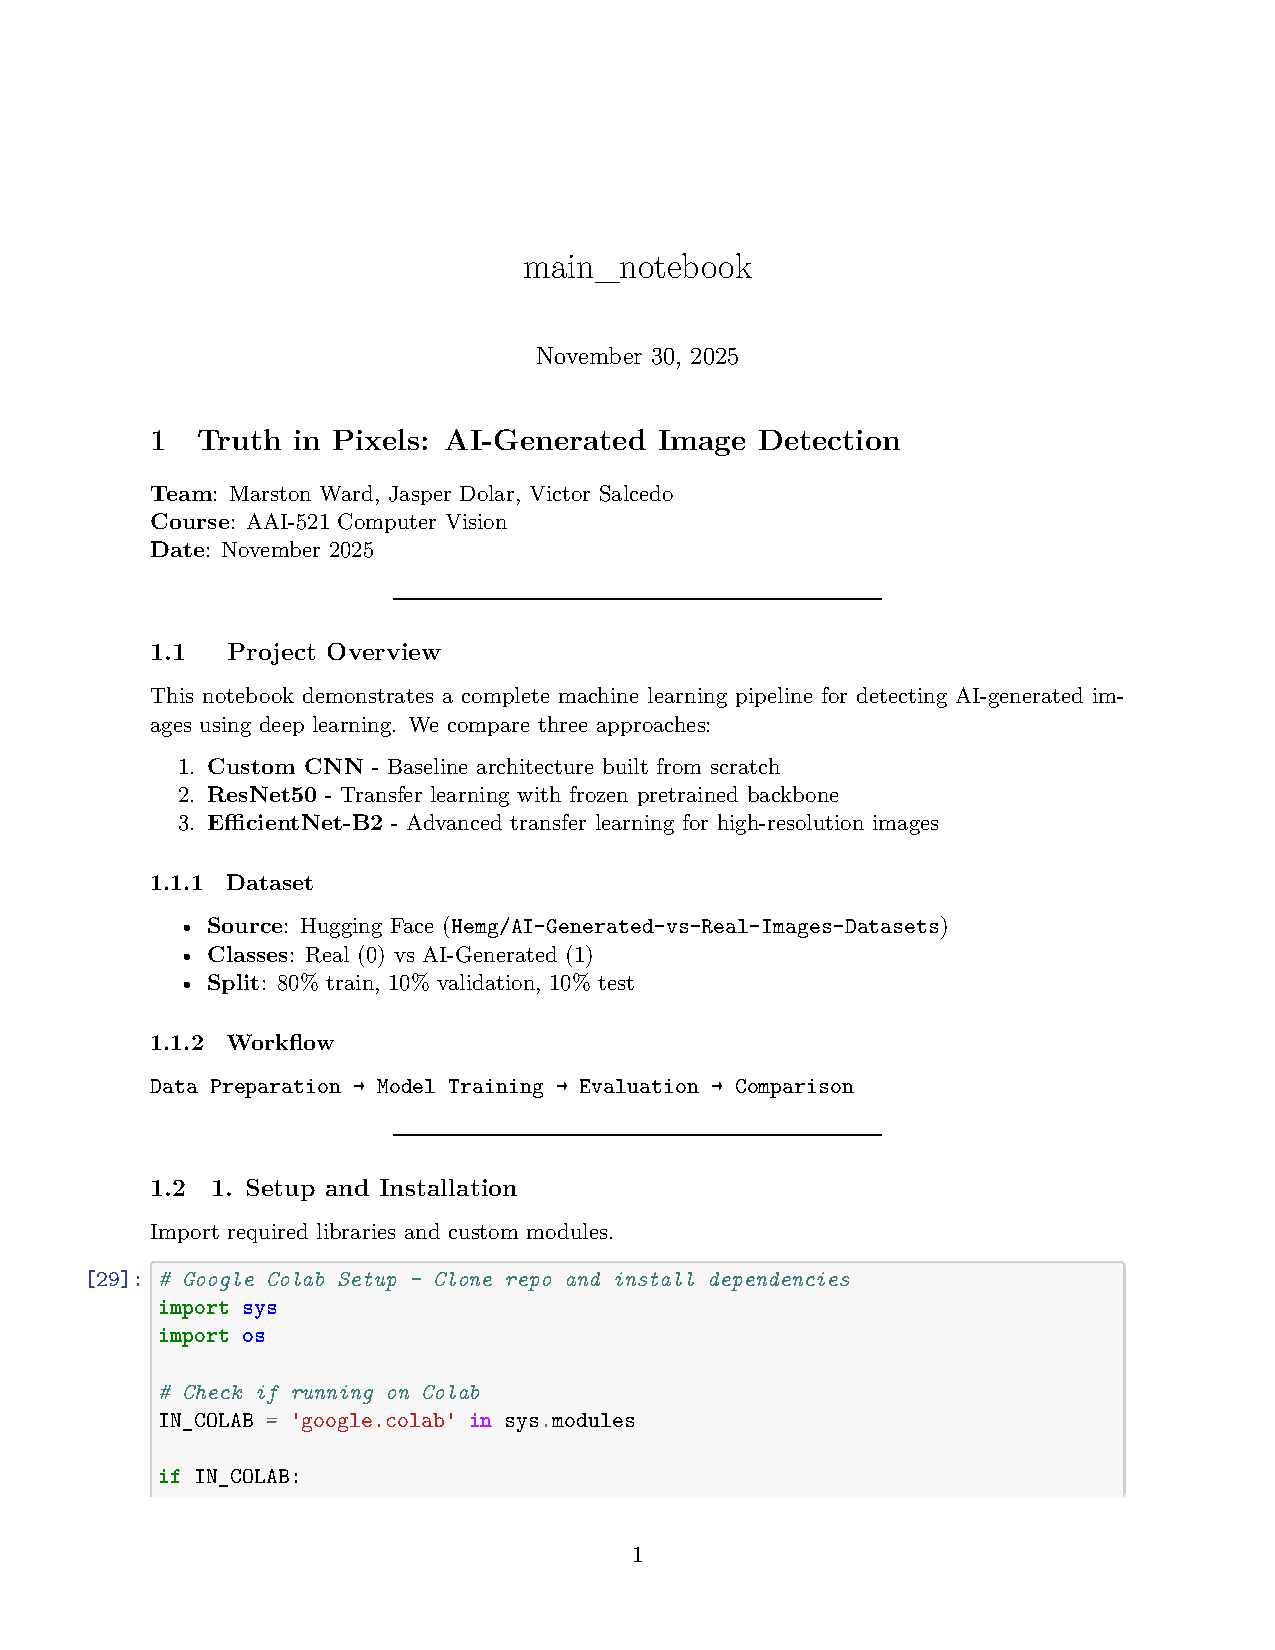
\includepdf[pages=-]{../main_notebook.pdf}

\section{Source Code}

This appendix contains the complete implementation code for the project, organized into five main modules.

\subsection{Data Loading Module (data.py)}

\begin{lstlisting}[style=pythonstyle]
"""
Data loading and preprocessing utilities.

Contains:
- HuggingFaceImageDataset: Custom PyTorch Dataset
- get_transforms: Create train/val data transforms
- prepare_data: Load and split dataset
"""

import random
from torch.utils.data import Dataset, DataLoader
from torchvision import transforms
from datasets import load_dataset


class HuggingFaceImageDataset(Dataset):
    """
    Custom PyTorch Dataset wrapper for Hugging Face images.
    
    Args:
        images (list): List of PIL images
        labels (list): List of corresponding labels (0=Real, 1=AI-Generated)
        transform (callable, optional): Optional transform to apply to images
    """
    def __init__(self, images, labels, transform=None):
        self.images = images
        self.labels = labels
        self.transform = transform
    
    def __len__(self):
        return len(self.images)
    
    def __getitem__(self, idx):
        image = self.images[idx]
        label = self.labels[idx]
        
        # Handle palette images with transparency
        if image.mode == 'P' and 'transparency' in image.info:
            image = image.convert('RGBA')
        
        if self.transform:
            image = self.transform(image)
        
        return image, label


def get_transforms(img_size=224, augment=True):
    """
    Get image transformation pipelines.
    
    Args:
        img_size (int): Target image size (default: 224)
        augment (bool): Apply data augmentation (for training)
    
    Returns:
        torchvision.transforms.Compose: Transform pipeline
    """
    # ImageNet normalization constants
    mean = [0.485, 0.456, 0.406]
    std = [0.229, 0.224, 0.225]
    
    if augment:
        # Training transforms with augmentation
        transform = transforms.Compose([
            transforms.Resize((img_size, img_size)),
            transforms.Lambda(lambda img: img.convert("RGB")),
            transforms.RandomHorizontalFlip(p=0.5),
            transforms.RandomRotation(10),
            transforms.ColorJitter(
                brightness=0.1,
                contrast=0.1,
                saturation=0.1,
                hue=0.05
            ),
            transforms.ToTensor(),
            transforms.Normalize(mean=mean, std=std)
        ])
    else:
        # Validation/test transforms (no augmentation)
        transform = transforms.Compose([
            transforms.Resize((img_size, img_size)),
            transforms.Lambda(lambda img: img.convert("RGB")),
            transforms.ToTensor(),
            transforms.Normalize(mean=mean, std=std)
        ])
    
    return transform


def prepare_data(dataset_name="Hemg/AI-Generated-vs-Real-Images-Datasets",
                 train_ratio=0.8,
                 val_ratio=0.1,
                 seed=42,
                 cache_dir="/root/.cache/huggingface/datasets"):
    """
    Load and split Hugging Face dataset.
    
    Args:
        dataset_name (str): Hugging Face dataset identifier
        train_ratio (float): Proportion for training (default: 0.8)
        val_ratio (float): Proportion for validation (default: 0.1)
        seed (int): Random seed for reproducibility (default: 42)
        cache_dir (str): Directory to cache downloaded dataset
    
    Returns:
        tuple: (train_images, train_labels, val_images, val_labels, 
                test_images, test_labels)
    """
    import os
    
    # Check if dataset is already cached
    cache_exists = os.path.exists(cache_dir) and any(
        dataset_name.replace('/', '___') in d 
        for d in os.listdir(cache_dir) 
        if os.path.isdir(os.path.join(cache_dir, d)))
    
    if cache_exists:
        print(f"Loading cached dataset '{dataset_name}'...")
    else:
        print(f"Downloading dataset '{dataset_name}'...")
        print("First download: ~2-3 min, then cached for future runs")
    
    dataset = load_dataset(dataset_name, token=False, cache_dir=cache_dir)
    print(f"Dataset loaded: {len(dataset['train']):,} total images")
    
    # Extract images and labels
    print("Preparing data splits...")
    images = [x['image'] for x in dataset['train']]
    labels = [x['label'] for x in dataset['train']]
    
    # Shuffle with seed
    random.seed(seed)
    combined = list(zip(images, labels))
    random.shuffle(combined)
    images, labels = zip(*combined)
    
    # Calculate split indices
    total_size = len(images)
    train_end = int(train_ratio * total_size)
    val_end = int((train_ratio + val_ratio) * total_size)
    
    # Split data
    train_images = images[:train_end]
    val_images = images[train_end:val_end]
    test_images = images[val_end:]
    
    train_labels = labels[:train_end]
    val_labels = labels[train_end:val_end]
    test_labels = labels[val_end:]
    
    return (train_images, train_labels,
            val_images, val_labels,
            test_images, test_labels)


def create_dataloaders(train_images, train_labels,
                      val_images, val_labels,
                      test_images, test_labels,
                      batch_size=32,
                      num_workers=2):
    """
    Create PyTorch DataLoaders from image/label lists.
    
    Args:
        train_images, train_labels: Training data
        val_images, val_labels: Validation data
        test_images, test_labels: Test data
        batch_size (int): Batch size for dataloaders (default: 32)
        num_workers (int): Number of worker processes (default: 2)
    
    Returns:
        tuple: (train_loader, val_loader, test_loader)
    """
    # Get transforms
    train_transform = get_transforms(augment=True)
    val_transform = get_transforms(augment=False)
    
    # Create datasets
    train_dataset = HuggingFaceImageDataset(
        train_images, train_labels, train_transform)
    val_dataset = HuggingFaceImageDataset(
        val_images, val_labels, val_transform)
    test_dataset = HuggingFaceImageDataset(
        test_images, test_labels, val_transform)
    
    # Create dataloaders
    train_loader = DataLoader(
        train_dataset,
        batch_size=batch_size,
        shuffle=True,
        num_workers=num_workers,
        pin_memory=True
    )
    
    val_loader = DataLoader(
        val_dataset,
        batch_size=batch_size,
        shuffle=False,
        num_workers=num_workers,
        pin_memory=True
    )
    
    test_loader = DataLoader(
        test_dataset,
        batch_size=batch_size,
        shuffle=False,
        num_workers=num_workers,
        pin_memory=True
    )
    
    return train_loader, val_loader, test_loader
\end{lstlisting}

\subsection{Model Architectures (models.py)}

\begin{lstlisting}[style=pythonstyle]
"""
Model architectures for AI-generated image detection.

Contains:
- CustomCNN: Baseline CNN with 3 conv layers
- get_resnet50: ResNet50 with transfer learning
- get_efficientnet_b2: EfficientNet-B2 with transfer learning
"""

import torch
import torch.nn as nn
import torch.nn.functional as F
from torchvision import models


class CustomCNN(nn.Module):
    """
    Custom CNN architecture for binary image classification.
    
    Architecture:
        - 3 convolutional layers (32, 64, 128 filters)
        - Batch normalization after each conv layer
        - MaxPooling after each conv block
        - Dropout for regularization
        - 2 fully connected layers
    
    Args:
        num_classes (int): Number of output classes (default: 1 for binary)
    """
    def __init__(self, num_classes=1):
        super(CustomCNN, self).__init__()
        
        # Convolutional layers
        self.conv1 = nn.Conv2d(3, 32, kernel_size=3, padding=1)
        self.bn1 = nn.BatchNorm2d(32)
        
        self.conv2 = nn.Conv2d(32, 64, kernel_size=3, padding=1)
        self.bn2 = nn.BatchNorm2d(64)
        
        self.conv3 = nn.Conv2d(64, 128, kernel_size=3, padding=1)
        self.bn3 = nn.BatchNorm2d(128)
        
        # Pooling and dropout
        self.pool = nn.MaxPool2d(2, 2)
        self.dropout = nn.Dropout(0.25)
        
        # Fully connected layers
        # After 3 pooling layers: 224/8 = 28, so 128 * 28 * 28
        self.fc1 = nn.Linear(128 * 28 * 28, 512)
        self.fc2 = nn.Linear(512, num_classes)
    
    def forward(self, x):
        # Conv block 1
        x = self.pool(F.relu(self.bn1(self.conv1(x))))
        
        # Conv block 2
        x = self.pool(F.relu(self.bn2(self.conv2(x))))
        
        # Conv block 3
        x = self.pool(F.relu(self.bn3(self.conv3(x))))
        
        # Flatten
        x = x.view(-1, 128 * 28 * 28)
        
        # Fully connected layers
        x = self.dropout(F.relu(self.fc1(x)))
        x = self.fc2(x)
        
        return x


def get_resnet50(num_classes=2, pretrained=True, freeze_backbone=True):
    """
    Get ResNet50 model with custom classifier for transfer learning.
    
    Args:
        num_classes (int): Number of output classes (default: 2)
        pretrained (bool): Use ImageNet pretrained weights (default: True)
        freeze_backbone (bool): Freeze all layers except classifier
    
    Returns:
        torch.nn.Module: ResNet50 model
    """
    # Load pretrained ResNet50
    if pretrained:
        model = models.resnet50(
            weights=models.ResNet50_Weights.IMAGENET1K_V1)
    else:
        model = models.resnet50(weights=None)
    
    # Freeze backbone if requested
    if freeze_backbone:
        for param in model.parameters():
            param.requires_grad = False
    
    # Replace final fully connected layer
    num_features = model.fc.in_features
    model.fc = nn.Linear(num_features, num_classes)
    
    return model


def get_efficientnet_b2(num_classes=2, pretrained=True, 
                        freeze_backbone=True):
    """
    Get EfficientNet-B2 model with custom classifier for transfer learning.
    
    Args:
        num_classes (int): Number of output classes (default: 2)
        pretrained (bool): Use ImageNet pretrained weights (default: True)
        freeze_backbone (bool): Freeze all layers except classifier
    
    Returns:
        torch.nn.Module: EfficientNet-B2 model
    """
    # Load pretrained EfficientNet-B2
    if pretrained:
        model = models.efficientnet_b2(
            weights=models.EfficientNet_B2_Weights.IMAGENET1K_V1)
    else:
        model = models.efficientnet_b2(weights=None)
    
    # Freeze backbone if requested
    if freeze_backbone:
        for param in model.parameters():
            param.requires_grad = False
    
    # Replace classifier head
    num_features = model.classifier[1].in_features
    model.classifier[1] = nn.Linear(num_features, num_classes)
    
    return model


def count_parameters(model):
    """
    Count trainable and total parameters in a model.
    
    Args:
        model (torch.nn.Module): PyTorch model
    
    Returns:
        tuple: (trainable_params, total_params)
    """
    trainable = sum(p.numel() for p in model.parameters() 
                   if p.requires_grad)
    total = sum(p.numel() for p in model.parameters())
    return trainable, total
\end{lstlisting}

\subsection{Training Module (training.py)}

\begin{lstlisting}[style=pythonstyle]
"""
Training and evaluation utilities.

Contains:
- Trainer: Main training class with AMP support
- evaluate_model: Model evaluation function
- save_checkpoint/load_checkpoint: Model persistence
"""

import os
import copy
import time
import torch
import torch.nn as nn
import torch.optim as optim
from pathlib import Path


class Trainer:
    """
    Training manager with automatic mixed precision (AMP) support.
    
    Args:
        model (torch.nn.Module): Model to train
        device (torch.device): Device to train on
        criterion (torch.nn.Module): Loss function
        optimizer (torch.optim.Optimizer): Optimizer
        use_amp (bool): Use automatic mixed precision (default: True)
    """
    def __init__(self, model, device, criterion, optimizer, use_amp=True):
        self.model = model
        self.device = device
        self.criterion = criterion
        self.optimizer = optimizer
        self.use_amp = use_amp
        
        # Initialize AMP scaler if using CUDA
        if use_amp and device.type == 'cuda':
            self.scaler = torch.amp.GradScaler('cuda')
        else:
            self.scaler = None
        
        # Training history
        self.history = {
            'train_loss': [],
            'train_acc': [],
            'val_loss': [],
            'val_acc': []
        }
        
        self.best_val_acc = 0.0
        self.best_model_wts = None
    
    def train_epoch(self, dataloader, verbose=True):
        """Train for one epoch."""
        self.model.train()
        running_loss = 0.0
        running_corrects = 0
        total = 0
        
        num_batches = len(dataloader)
        print_every = max(num_batches // 10, 100)
        
        for batch_idx, (images, labels) in enumerate(dataloader):
            images = images.to(self.device, non_blocking=True)
            labels = labels.to(self.device, non_blocking=True)
            
            self.optimizer.zero_grad()
            
            # Forward pass with AMP
            if self.scaler is not None:
                with torch.amp.autocast('cuda'):
                    outputs = self.model(images)
                    if outputs.dim() == 2 and outputs.size(1) == 1:
                        labels_for_loss = labels.float().unsqueeze(1)
                    else:
                        labels_for_loss = labels
                    loss = self.criterion(outputs, labels_for_loss)
                
                # Backward pass with scaler
                self.scaler.scale(loss).backward()
                self.scaler.step(self.optimizer)
                self.scaler.update()
            else:
                outputs = self.model(images)
                if outputs.dim() == 2 and outputs.size(1) == 1:
                    labels_for_loss = labels.float().unsqueeze(1)
                else:
                    labels_for_loss = labels
                loss = self.criterion(outputs, labels_for_loss)
                loss.backward()
                self.optimizer.step()
            
            # Calculate accuracy
            batch_size = labels.size(0)
            
            if outputs.dim() == 1 or outputs.size(1) == 1:
                preds = (torch.sigmoid(outputs.squeeze()) > 0.5).long()
            else:
                _, preds = torch.max(outputs, 1)
            
            running_loss += loss.item() * batch_size
            running_corrects += torch.sum(preds == labels).item()
            total += batch_size
            
            # Print progress
            if verbose and (batch_idx + 1) % print_every == 0:
                batch_acc = running_corrects / total
                avg_loss = running_loss / total
                print(f"  [{batch_idx+1:4d}/{num_batches}] "
                      f"Loss: {avg_loss:.4f} | Acc: {batch_acc:.4f}")
        
        epoch_loss = running_loss / total
        epoch_acc = running_corrects / total
        
        return epoch_loss, epoch_acc
    
    def validate(self, dataloader):
        """Validate model on validation set."""
        self.model.eval()
        running_loss = 0.0
        running_corrects = 0
        total = 0
        
        with torch.no_grad():
            for images, labels in dataloader:
                images = images.to(self.device, non_blocking=True)
                labels = labels.to(self.device, non_blocking=True)
                
                outputs = self.model(images)
                if outputs.dim() == 2 and outputs.size(1) == 1:
                    labels_for_loss = labels.float().unsqueeze(1)
                else:
                    labels_for_loss = labels
                loss = self.criterion(outputs, labels_for_loss)
                
                batch_size = labels.size(0)
                
                if outputs.dim() == 1 or outputs.size(1) == 1:
                    preds = (torch.sigmoid(outputs.squeeze()) > 0.5).long()
                else:
                    _, preds = torch.max(outputs, 1)
                
                running_loss += loss.item() * batch_size
                running_corrects += torch.sum(preds == labels).item()
                total += batch_size
        
        epoch_loss = running_loss / total
        epoch_acc = running_corrects / total
        
        return epoch_loss, epoch_acc
    
    def fit(self, train_loader, val_loader, num_epochs, 
            save_path=None, verbose=True):
        """Train model for multiple epochs."""
        start_time = time.time()
        
        for epoch in range(num_epochs):
            if verbose:
                print(f"\\nEpoch {epoch+1}/{num_epochs}")
                print("-" * 40)
            
            # Train
            train_loss, train_acc = self.train_epoch(
                train_loader, verbose=verbose)
            self.history['train_loss'].append(train_loss)
            self.history['train_acc'].append(train_acc)
            
            # Validate
            val_loss, val_acc = self.validate(val_loader)
            self.history['val_loss'].append(val_loss)
            self.history['val_acc'].append(val_acc)
            
            if verbose:
                print(f"Train Loss: {train_loss:.4f} | "
                      f"Train Acc: {train_acc:.4f}")
                print(f"Val   Loss: {val_loss:.4f} | "
                      f"Val   Acc: {val_acc:.4f}")
            
            # Save best model
            if val_acc > self.best_val_acc:
                self.best_val_acc = val_acc
                self.best_model_wts = copy.deepcopy(
                    self.model.state_dict())
                
                if save_path:
                    save_checkpoint(self.model, save_path)
                    if verbose:
                        print(f"Saved best model "
                              f"(val_acc: {val_acc:.4f})")
        
        # Load best weights
        if self.best_model_wts is not None:
            self.model.load_state_dict(self.best_model_wts)
        
        elapsed = time.time() - start_time
        if verbose:
            print(f"\\nTraining complete in {elapsed:.0f}s")
            print(f"Best validation accuracy: {self.best_val_acc:.4f}")
        
        return self.history


def evaluate_model(model, dataloader, device):
    """Evaluate model on a dataset."""
    model.eval()
    all_preds = []
    all_labels = []
    correct = 0
    total = 0
    
    with torch.no_grad():
        for images, labels in dataloader:
            images = images.to(device)
            labels = labels.to(device)
            
            outputs = model(images)
            _, preds = torch.max(outputs, 1)
            
            all_preds.extend(preds.cpu().numpy())
            all_labels.extend(labels.cpu().numpy())
            
            correct += (preds == labels).sum().item()
            total += labels.size(0)
    
    accuracy = correct / total
    return accuracy, all_preds, all_labels


def save_checkpoint(model, path):
    """Save model checkpoint."""
    Path(path).parent.mkdir(parents=True, exist_ok=True)
    torch.save(model.state_dict(), path)


def load_checkpoint(model, path, device):
    """Load model checkpoint."""
    model.load_state_dict(torch.load(path, map_location=device))
    return model
\end{lstlisting}

\subsection{Visualization Module (visualization.py)}

\begin{lstlisting}[style=pythonstyle]
"""
Visualization utilities for model evaluation and analysis.

Contains:
- plot_training_history: Plot loss and accuracy curves
- plot_confusion_matrix: Display confusion matrix
- compare_models: Side-by-side model comparison
"""

import numpy as np
import matplotlib.pyplot as plt
import seaborn as sns
from sklearn.metrics import confusion_matrix, classification_report


def plot_training_history(history, title="Training History"):
    """Plot training and validation loss/accuracy curves."""
    fig, axes = plt.subplots(1, 2, figsize=(14, 5))
    
    # Loss plot
    axes[0].plot(history['train_loss'], label='Train Loss', marker='o')
    axes[0].plot(history['val_loss'], label='Val Loss', marker='s')
    axes[0].set_xlabel('Epoch')
    axes[0].set_ylabel('Loss')
    axes[0].set_title('Loss Curves')
    axes[0].legend()
    axes[0].grid(alpha=0.3)
    
    # Accuracy plot
    axes[1].plot(history['train_acc'], label='Train Acc', marker='o')
    axes[1].plot(history['val_acc'], label='Val Acc', marker='s')
    axes[1].set_xlabel('Epoch')
    axes[1].set_ylabel('Accuracy')
    axes[1].set_title('Accuracy Curves')
    axes[1].legend()
    axes[1].grid(alpha=0.3)
    
    plt.suptitle(title, fontsize=16, fontweight='bold')
    plt.tight_layout()
    plt.show()


def plot_confusion_matrix(y_true, y_pred, 
                         class_names=['Real', 'AI-Generated'], 
                         title='Confusion Matrix'):
    """Plot confusion matrix heatmap."""
    cm = confusion_matrix(y_true, y_pred)
    
    plt.figure(figsize=(8, 6))
    sns.heatmap(cm, annot=True, fmt='d', cmap='Blues',
                xticklabels=class_names,
                yticklabels=class_names,
                cbar_kws={'label': 'Count'})
    plt.title(title, fontsize=16, fontweight='bold')
    plt.xlabel('Predicted', fontsize=12)
    plt.ylabel('Actual', fontsize=12)
    plt.tight_layout()
    plt.show()


def compare_models(results_dict, metric='accuracy'):
    """Create bar chart comparing multiple models."""
    models = list(results_dict.keys())
    values = list(results_dict.values())
    
    plt.figure(figsize=(10, 6))
    colors = ['#3498db', '#e74c3c', '#2ecc71']
    bars = plt.bar(models, values, color=colors[:len(models)], 
                   edgecolor='black', linewidth=1.5)
    
    # Add value labels on bars
    for bar in bars:
        height = bar.get_height()
        plt.text(bar.get_x() + bar.get_width()/2., height,
                f'{height:.4f}',
                ha='center', va='bottom', fontsize=12, 
                fontweight='bold')
    
    plt.ylabel(metric.capitalize(), fontsize=14)
    plt.title(f'Model Comparison - {metric.capitalize()}', 
              fontsize=16, fontweight='bold')
    plt.ylim(0, 1.1)
    plt.grid(axis='y', alpha=0.3)
    plt.tight_layout()
    plt.show()
\end{lstlisting}

\subsection{Exploratory Data Analysis Module (eda.py)}

\begin{lstlisting}[style=pythonstyle]
"""
Exploratory Data Analysis (EDA) utilities.

Contains functions for visualizing and analyzing 
the dataset before training.
"""

import random
import numpy as np
import matplotlib.pyplot as plt
from collections import Counter


def analyze_class_distribution(labels, 
                               class_names=['Real', 'AI-Generated']):
    """Analyze and print class distribution statistics."""
    unique, counts = np.unique(labels, return_counts=True)
    total = len(labels)
    
    stats = {}
    print("Class Distribution:")
    for label, count in zip(unique, counts):
        class_name = class_names[label] if label < len(class_names) \
                     else f"Class {label}"
        percentage = (count / total) * 100
        stats[class_name] = {'count': count, 'percentage': percentage}
        print(f"   {class_name}: {count:,} images ({percentage:.1f}%)")
    
    return stats


def plot_class_distribution(labels, 
                           class_names=['Real', 'AI-Generated'], 
                           title='Class Distribution', 
                           figsize=(8, 5)):
    """Plot class distribution as a bar chart."""
    unique, counts = np.unique(labels, return_counts=True)
    
    plt.figure(figsize=figsize)
    colors = ['#3498db', '#e74c3c', '#2ecc71', '#f39c12'][:len(unique)]
    bars = plt.bar(class_names[:len(unique)], counts, color=colors, 
                   edgecolor='black', linewidth=1.5)
    
    plt.title(title, fontsize=16, fontweight='bold')
    plt.ylabel('Number of Images', fontsize=12)
    plt.xlabel('Class', fontsize=12)
    plt.grid(axis='y', alpha=0.3)
    
    # Add count labels on bars
    for bar in bars:
        height = bar.get_height()
        plt.text(bar.get_x() + bar.get_width()/2., height,
                f'{int(height):,}',
                ha='center', va='bottom', fontsize=12, 
                fontweight='bold')
    
    plt.tight_layout()
    plt.show()


def visualize_samples(images, labels, 
                     class_names=['Real', 'AI-Generated'],
                     n_per_class=4, figsize=(16, 8), seed=None):
    """Display sample images from each class in a grid."""
    if seed is not None:
        random.seed(seed)
    
    # Separate images by class
    classes = {}
    for img, lbl in zip(images, labels):
        if lbl not in classes:
            classes[lbl] = []
        classes[lbl].append(img)
    
    # Create subplot grid
    n_classes = len(classes)
    fig, axes = plt.subplots(n_classes, n_per_class, figsize=figsize)
    
    # Plot samples for each class
    for class_idx, (label, class_images) in enumerate(
            sorted(classes.items())):
        class_name = class_names[label] if label < len(class_names) \
                     else f"Class {label}"
        color = ['#3498db', '#e74c3c', '#2ecc71', '#f39c12'][label % 4]
        
        for img_idx in range(n_per_class):
            if img_idx < len(class_images):
                sample_img = random.choice(class_images)
                axes[class_idx, img_idx].imshow(sample_img)
            else:
                axes[class_idx, img_idx].axis('off')
            
            if img_idx == 0:
                axes[class_idx, img_idx].set_ylabel(
                    class_name, fontsize=12, fontweight='bold', 
                    color=color)
            
            axes[class_idx, img_idx].axis('off')
    
    plt.tight_layout()
    plt.show()


def dataset_summary(train_images, train_labels, 
                   val_images, val_labels, 
                   test_images, test_labels, 
                   class_names=['Real', 'AI-Generated']):
    """Print comprehensive dataset summary statistics."""
    total_size = len(train_images) + len(val_images) + len(test_images)
    
    print("\\n" + "="*60)
    print("DATASET SUMMARY")
    print("="*60)
    print(f"\\nTotal Images: {total_size:,}")
    print(f"\\nSplit:")
    print(f"   Training:   {len(train_images):,} images "
          f"({len(train_images)/total_size*100:.1f}%)")
    print(f"   Validation: {len(val_images):,} images "
          f"({len(val_images)/total_size*100:.1f}%)")
    print(f"   Test:       {len(test_images):,} images "
          f"({len(test_images)/total_size*100:.1f}%)")
    
    print("="*60)
\end{lstlisting}

\end{document}